

\documentclass[nooutcomes]{ximera}

\graphicspath{
  {./}
  {1-1QuantitativeReasoning/}
  {1-2RelationsAndGraphs/}
  {1-3ChangingInTandem/}
  {2-1LinearEquations/}
  {2-2LinearModeling/}
  {2-3ExponentialModeling/}
  {3-1WhatIsAFunction/}
  {3-2FunctionProperties/}
  {3-3AverageRatesOfChange/}
  {4-1BuildingNewFunctions/}
  {4-2Polynomials/}
  {5-1RationalFunctions/}
   {5-2ExponentialFunctions/}
  {6-1Domain/}
  {6-2Range/}
  {6-3CompositionOfFunctions/}
  {6-4FunctionTransformations/}
  {7-1ZerosOfFunctions/}
  {7-XZerosOfPolynomials/}
  {7-2ZerosOfFamousFunctions/}
  {8-1SystemsOfEquations/}
  {6-5FunctionTransformationsProject/}
  {1-1QuantitativeReasoning/exercises/}
  {1-2RelationsAndGraphs/exercises/}
  {../1-3ChangingInTandem/exercises/}
  {../2-1LinearEquations/exercises/}
  {../2-2LinearModeling/exercises/}
  {../2-3ExponentialModeling/exercises/}
  {../3-1WhatIsAFunction/exercises/}
  {../3-2FunctionProperties/exercises/}
  {../3-3AverageRatesOfChange/exercises/}
  {../5-2ExponentialFunctions/exercises/}
  {../4-1BuildingNewFunctions/exercises/}
  {../4-2Polynomials/exercises/}
  {../5-1RationalFunctions/exercises/}
  {../6-1Domain/exercises/}
  {../6-2Range/exercises/}
  {../6-3CompositionOfFunctions/exercises/}
  {../7-1ZerosOfFunctions/exercises/}
  {../7-XZerosOfPolynomials/exercises/}
  {../7-2ZerosOfFamousFunctions/exercises/}
  {../6-4FunctionTransformations/exercises/}
  {../8-1SystemsOfEquations/exercises/}
  {../6-3FunctionTransformationsProject/exercises/}
}

\DeclareGraphicsExtensions{.pdf,.png,.jpg,.eps}

\newcommand{\mooculus}{\textsf{\textbf{MOOC}\textnormal{\textsf{ULUS}}}}

\usepackage[makeroom]{cancel} %% for strike outs

\ifxake
\else
\usepackage[most]{tcolorbox}
\fi


%\typeout{************************************************}
%\typeout{New Environments}
%\typeout{************************************************}

%% to fix for web can be removed when deployed offically with ximera2
\let\image\relax\let\endimage\relax
\NewEnviron{image}{% 
  \begin{center}\BODY\end{center}% center
}



\NewEnviron{folder}{
      \addcontentsline{toc}{section}{\textbf{\BODY}}
}

\ifxake
\let\summary\relax
\let\endsummary\relax
\newtheorem*{summary}{Summary}
\newtheorem*{callout}{Callout}
\newtheorem*{overview}{Overview}
\newtheorem*{objectives}{Objectives}
\newtheorem*{motivatingQuestions}{Motivating Questions}
\newtheorem*{MM}{Metacognitive Moment}
      
%% NEEDED FOR XIMERA 2
%\ximerizedEnvironment{summary}
%\ximerizedEnvironment{callout}
%\ximerizedEnvironment{overview} 
%\ximerizedEnvironment{objectives}
%\ximerizedEnvironment{motivatingQuestions}
%\ximerizedEnvironment{MM}
\else
%% CALLOUT
\NewEnviron{callout}{
  \begin{tcolorbox}[colback=blue!5, breakable,pad at break*=1mm]
      \BODY
  \end{tcolorbox}
}
%% MOTIVATING QUESTIONS
\NewEnviron{motivatingQuestions}{
  \begin{tcolorbox}[ breakable,pad at break*=1mm]
    \textbf{\Large Motivating Questions}\hfill
    %\begin{itemize}[label=\textbullet]
      \BODY
    %\end{itemize}
  \end{tcolorbox}
}
%% OBJECTIVES
\NewEnviron{objectives}{  
    \vspace{.5in}
      %\begin{tcolorbox}[colback=orange!5, breakable,pad at break*=1mm]
    \textbf{\Large Learning Objectives}
    \begin{itemize}[label=\textbullet]
      \BODY
    \end{itemize}
    %\end{tcolorbox}
}
%% DEFINITION
\let\definition\relax
\let\enddefinition\relax
\NewEnviron{definition}{
  \begin{tcolorbox}[ breakable,pad at break*=1mm]
    \noindent\textbf{Definition}~
      \BODY
  \end{tcolorbox}
}
%% OVERVIEW
\let\overview\relax
\let\overview\relax
\NewEnviron{overview}{
  \begin{tcolorbox}[ breakable,pad at break*=1mm]
    \textbf{\Large Overview}
    %\begin{itemize}[label=\textbullet] %% breaks Xake
      \BODY
    %\end{itemize}
  \end{tcolorbox}
}
%% SUMMARY
\let\summary\relax
\let\endsummary\relax
\NewEnviron{summary}{
  \begin{tcolorbox}[ breakable,pad at break*=1mm]
    \textbf{\Large Summary}
    %\begin{itemize}[label=\textbullet] %% breaks Xake
      \BODY
    %\end{itemize}
  \end{tcolorbox}
}
%% REMARK
\let\remark\relax
\let\endremark\relax
\NewEnviron{remark}{
  \begin{tcolorbox}[colback=green!5, breakable,pad at break*=1mm]
    \noindent\textbf{Remark}~
      \BODY
  \end{tcolorbox}
}
%% EXPLANATION
\let\explanation\relax
\let\endexplanation\relax
\NewEnviron{explanation}{
    \normalfont
    \noindent\textbf{Explanation}~
      \BODY
}
%% EXPLORATION
\let\exploration\relax
\let\endexploration\relax
\NewEnviron{exploration}{
  \begin{tcolorbox}[colback=yellow!10, breakable,pad at break*=1mm]
    \noindent\textbf{Exploration}~
      \BODY
  \end{tcolorbox}
}
%% METACOGNITIVE MOMENTS
\let\MM\relax
\let\endMM\relax
\NewEnviron{MM}{
  \begin{tcolorbox}[colback=pink!15, breakable,pad at break*=1mm]
    \noindent\textbf{Metacognitive Moment}~
      \BODY
  \end{tcolorbox}
}


\fi





%Notes on what envirnoment to use:  Example with Explanation in text; if they are supposed to answer- Problem; no answer - Exploration


%\typeout{************************************************}
%% Header and footers
%\typeout{************************************************}

\newcommand{\licenseAcknowledgement}{Licensed under Creative Commons 4.0}
\newcommand{\licenseAPC}{\renewcommand{\licenseAcknowledgement}{\textbf{Acknowledgements:} Active Prelude to Calculus (https://activecalculus.org/prelude) }}
\newcommand{\licenseSZ}{\renewcommand{\licenseAcknowledgement}{\textbf{Acknowledgements:} Stitz Zeager Open Source Mathematics (https://www.stitz-zeager.com/) }}
\newcommand{\licenseAPCSZ}{\renewcommand{\licenseAcknowledgement}{\textbf{Acknowledgements:} Active Prelude to Calculus (https://activecalculus.org/prelude) and Stitz Zeager Open Source Mathematics (https://www.stitz-zeager.com/) }}
\newcommand{\licenseORCCA}{\renewcommand{\licenseAcknowledgement}{\textbf{Acknowledgements:}Original source material, products with readable and accessible
math content, and other information freely available at pcc.edu/orcca.}}
\newcommand{\licenseY}{\renewcommand{\licenseAcknowledgement}{\textbf{Acknowledgements:} Yoshiwara Books (https://yoshiwarabooks.org/)}}
\newcommand{\licenseOS}{\renewcommand{\licenseAcknowledgement}{\textbf{Acknowledgements:} OpenStax College Algebra (https://openstax.org/details/books/college-algebra)}}
\newcommand{\licenseAPCSZCSCC}{\renewcommand{\licenseAcknowledgement}{\textbf{Acknowledgements:} Active Prelude to Calculus (https://activecalculus.org/prelude), Stitz Zeager Open Source Mathematics (https://www.stitz-zeager.com/), CSCC PreCalculus and Calculus texts (https://ximera.osu.edu/csccmathematics)}}

\ifxake\else %% do nothing on the website
\usepackage{fancyhdr}
\pagestyle{fancy}
\fancyhf{}
\fancyhead[R]{\sectionmark}
\fancyfoot[L]{\thepage}
\fancyfoot[C]{\licenseAcknowledgement}
\renewcommand{\headrulewidth}{0pt}
\renewcommand{\footrulewidth}{0pt}
\fi

%%%%%%%%%%%%%%%%



%\typeout{************************************************}
%\typeout{Table of Contents}
%\typeout{************************************************}


%% Edit this to change the font style
\newcommand{\sectionHeadStyle}{\sffamily\bfseries}


\makeatletter

%% part uses arabic numerals
\renewcommand*\thepart{\arabic{part}}


\ifxake\else
\renewcommand\chapterstyle{%
  \def\maketitle{%
    \addtocounter{titlenumber}{1}%
    \pagestyle{fancy}
    \phantomsection
    \addcontentsline{toc}{section}{\textbf{\thepart.\thetitlenumber\hspace{1em}\@title}}%
                    {\flushleft\small\sectionHeadStyle\@pretitle\par\vspace{-1.5em}}%
                    {\flushleft\LARGE\sectionHeadStyle\thepart.\thetitlenumber\hspace{1em}\@title \par }%
                    {\setcounter{problem}{0}\setcounter{sectiontitlenumber}{0}}%
                    \par}}





\renewcommand\sectionstyle{%
  \def\maketitle{%
    \addtocounter{sectiontitlenumber}{1}
    \pagestyle{fancy}
    \phantomsection
    \addcontentsline{toc}{subsection}{\thepart.\thetitlenumber.\thesectiontitlenumber\hspace{1em}\@title}%
    {\flushleft\small\sectionHeadStyle\@pretitle\par\vspace{-1.5em}}%
    {\flushleft\Large\sectionHeadStyle\thepart.\thetitlenumber.\thesectiontitlenumber\hspace{1em}\@title \par}%
    %{\setcounter{subsectiontitlenumber}{0}}%
    \par}}



\renewcommand\section{\@startsection{paragraph}{10}{\z@}%
                                     {-3.25ex\@plus -1ex \@minus -.2ex}%
                                     {1.5ex \@plus .2ex}%
                                     {\normalfont\large\sectionHeadStyle}}
\renewcommand\subsection{\@startsection{subparagraph}{10}{\z@}%
                                    {3.25ex \@plus1ex \@minus.2ex}%
                                    {-1em}%
                                    {\normalfont\normalsize\sectionHeadStyle}}

\fi

%% redefine Part
\renewcommand\part{%
   {\setcounter{titlenumber}{0}}
  \if@openright
    \cleardoublepage
  \else
    \clearpage
  \fi
  \thispagestyle{plain}%
  \if@twocolumn
    \onecolumn
    \@tempswatrue
  \else
    \@tempswafalse
  \fi
  \null\vfil
  \secdef\@part\@spart}

\def\@part[#1]#2{%
    \ifnum \c@secnumdepth >-2\relax
      \refstepcounter{part}%
      \addcontentsline{toc}{part}{\thepart\hspace{1em}#1}%
    \else
      \addcontentsline{toc}{part}{#1}%
    \fi
    \markboth{}{}%
    {\centering
     \interlinepenalty \@M
     \normalfont
     \ifnum \c@secnumdepth >-2\relax
       \huge\sffamily\bfseries \partname\nobreakspace\thepart
       \par
       \vskip 20\p@
     \fi
     \Huge \bfseries #2\par}%
    \@endpart}
\def\@spart#1{%
    {\centering
     \interlinepenalty \@M
     \normalfont
     \Huge \bfseries #1\par}%
    \@endpart}
\def\@endpart{\vfil\newpage
              \if@twoside
               \if@openright
                \null
                \thispagestyle{empty}%
                \newpage
               \fi
              \fi
              \if@tempswa
                \twocolumn
                \fi}



\makeatother





%\typeout{************************************************}
%\typeout{Stuff from Ximera}
%\typeout{************************************************}



\usepackage{array}  %% This is for typesetting long division
\setlength{\extrarowheight}{+.1cm}
\newdimen\digitwidth
\settowidth\digitwidth{9}
\def\divrule#1#2{
\noalign{\moveright#1\digitwidth
\vbox{\hrule width#2\digitwidth}}}





\newcommand{\RR}{\mathbb R}
\newcommand{\R}{\mathbb R}
\newcommand{\N}{\mathbb N}
\newcommand{\Z}{\mathbb Z}

\newcommand{\sagemath}{\textsf{SageMath}}


\def\d{\,d}
%\renewcommand{\d}{\mathop{}\!d}
\newcommand{\dd}[2][]{\frac{\d #1}{\d #2}}
\newcommand{\pp}[2][]{\frac{\partial #1}{\partial #2}}
\renewcommand{\l}{\ell}
\newcommand{\ddx}{\frac{d}{\d x}}



%\newcommand{\unit}{\,\mathrm}
\newcommand{\unit}{\mathop{}\!\mathrm}
\newcommand{\eval}[1]{\bigg[ #1 \bigg]}
\newcommand{\seq}[1]{\left( #1 \right)}
\renewcommand{\epsilon}{\varepsilon}
\renewcommand{\phi}{\varphi}


\renewcommand{\iff}{\Leftrightarrow}

\DeclareMathOperator{\arccot}{arccot}
\DeclareMathOperator{\arcsec}{arcsec}
\DeclareMathOperator{\arccsc}{arccsc}
\DeclareMathOperator{\sign}{sign}


%\DeclareMathOperator{\divergence}{divergence}
%\DeclareMathOperator{\curl}[1]{\grad\cross #1}
\newcommand{\lto}{\mathop{\longrightarrow\,}\limits}

\renewcommand{\bar}{\overline}

\colorlet{textColor}{black}
\colorlet{background}{white}
\colorlet{penColor}{blue!50!black} % Color of a curve in a plot
\colorlet{penColor2}{red!50!black}% Color of a curve in a plot
\colorlet{penColor3}{red!50!blue} % Color of a curve in a plot
\colorlet{penColor4}{green!50!black} % Color of a curve in a plot
\colorlet{penColor5}{orange!80!black} % Color of a curve in a plot
\colorlet{penColor6}{yellow!70!black} % Color of a curve in a plot
\colorlet{fill1}{penColor!20} % Color of fill in a plot
\colorlet{fill2}{penColor2!20} % Color of fill in a plot
\colorlet{fillp}{fill1} % Color of positive area
\colorlet{filln}{penColor2!20} % Color of negative area
\colorlet{fill3}{penColor3!20} % Fill
\colorlet{fill4}{penColor4!20} % Fill
\colorlet{fill5}{penColor5!20} % Fill
\colorlet{gridColor}{gray!50} % Color of grid in a plot

\newcommand{\surfaceColor}{violet}
\newcommand{\surfaceColorTwo}{redyellow}
\newcommand{\sliceColor}{greenyellow}




\pgfmathdeclarefunction{gauss}{2}{% gives gaussian
  \pgfmathparse{1/(#2*sqrt(2*pi))*exp(-((x-#1)^2)/(2*#2^2))}%
}





%\typeout{************************************************}
%\typeout{ORCCA Preamble.Tex}
%\typeout{************************************************}


%% \usepackage{geometry}
%% \geometry{letterpaper,total={408pt,9.0in}}
%% Custom Page Layout Adjustments (use latex.geometry)
%% \usepackage{amsmath,amssymb}
%% \usepackage{pgfplots}
\usepackage{pifont}                                         %needed for symbols, s.a. airplane symbol
\usetikzlibrary{positioning,fit,backgrounds}                %needed for nested diagrams
\usetikzlibrary{calc,trees,positioning,arrows,fit,shapes}   %needed for set diagrams
\usetikzlibrary{decorations.text}                           %needed for text following a curve
\usetikzlibrary{arrows,arrows.meta}                         %needed for open/closed intervals
\usetikzlibrary{positioning,3d,shapes.geometric}            %needed for 3d number sets tower

%% NEEDED FOR XIMERA 1
%\usetkzobj{all}       %NO LONGER VALID
%%%%%%%%%%%%%%

\usepackage{tikz-3dplot}
\usepackage{tkz-euclide}                     %needed for triangle diagrams
\usepgfplotslibrary{fillbetween}                            %shade regions of a plot
\usetikzlibrary{shadows}                                    %function diagrams
\usetikzlibrary{positioning}                                %function diagrams
\usetikzlibrary{shapes}                                     %function diagrams
%%% global colors from https://www.pcc.edu/web-services/style-guide/basics/color/ %%%
\definecolor{ruby}{HTML}{9E0C0F}
\definecolor{turquoise}{HTML}{008099}
\definecolor{emerald}{HTML}{1c8464}
\definecolor{amber}{HTML}{c7502a}
\definecolor{amethyst}{HTML}{70485b}
\definecolor{sapphire}{HTML}{263c53}
\colorlet{firstcolor}{sapphire}
\colorlet{secondcolor}{turquoise}
\colorlet{thirdcolor}{emerald}
\colorlet{fourthcolor}{amber}
\colorlet{fifthcolor}{amethyst}
\colorlet{sixthcolor}{ruby}
\colorlet{highlightcolor}{green!50!black}
\colorlet{graphbackground}{white}
\colorlet{wood}{brown!60!white}
%%% curve, dot, and graph custom styles %%%
\pgfplotsset{firstcurve/.style      = {color=firstcolor,  mark=none, line width=1pt, {Kite}-{Kite}, solid}}
\pgfplotsset{secondcurve/.style     = {color=secondcolor, mark=none, line width=1pt, {Kite}-{Kite}, solid}}
\pgfplotsset{thirdcurve/.style      = {color=thirdcolor,  mark=none, line width=1pt, {Kite}-{Kite}, solid}}
\pgfplotsset{fourthcurve/.style     = {color=fourthcolor, mark=none, line width=1pt, {Kite}-{Kite}, solid}}
\pgfplotsset{fifthcurve/.style      = {color=fifthcolor,  mark=none, line width=1pt, {Kite}-{Kite}, solid}}
\pgfplotsset{highlightcurve/.style  = {color=highlightcolor,  mark=none, line width=5pt, -, opacity=0.3}}   % thick, opaque curve for highlighting
\pgfplotsset{asymptote/.style       = {color=gray, mark=none, line width=1pt, <->, dashed}}
\pgfplotsset{symmetryaxis/.style    = {color=gray, mark=none, line width=1pt, <->, dashed}}
\pgfplotsset{guideline/.style       = {color=gray, mark=none, line width=1pt, -}}
\tikzset{guideline/.style           = {color=gray, mark=none, line width=1pt, -}}
\pgfplotsset{altitude/.style        = {dashed, color=gray, thick, mark=none, -}}
\tikzset{altitude/.style            = {dashed, color=gray, thick, mark=none, -}}
\pgfplotsset{radius/.style          = {dashed, thick, mark=none, -}}
\tikzset{radius/.style              = {dashed, thick, mark=none, -}}
\pgfplotsset{rightangle/.style      = {color=gray, mark=none, -}}
\tikzset{rightangle/.style          = {color=gray, mark=none, -}}
\pgfplotsset{closedboundary/.style  = {color=black, mark=none, line width=1pt, {Kite}-{Kite},solid}}
\tikzset{closedboundary/.style      = {color=black, mark=none, line width=1pt, {Kite}-{Kite},solid}}
\pgfplotsset{openboundary/.style    = {color=black, mark=none, line width=1pt, {Kite}-{Kite},dashed}}
\tikzset{openboundary/.style        = {color=black, mark=none, line width=1pt, {Kite}-{Kite},dashed}}
\tikzset{verticallinetest/.style    = {color=gray, mark=none, line width=1pt, <->,dashed}}
\pgfplotsset{soliddot/.style        = {color=firstcolor,  mark=*, only marks}}
\pgfplotsset{hollowdot/.style       = {color=firstcolor,  mark=*, only marks, fill=graphbackground}}
\pgfplotsset{blankgraph/.style      = {xmin=-10, xmax=10,
                                        ymin=-10, ymax=10,
                                        axis line style={-, draw opacity=0 },
                                        axis lines=box,
                                        major tick length=0mm,
                                        xtick={-10,-9,...,10},
                                        ytick={-10,-9,...,10},
                                        grid=major,
                                        grid style={solid,gray!20},
                                        xticklabels={,,},
                                        yticklabels={,,},
                                        minor xtick=,
                                        minor ytick=,
                                        xlabel={},ylabel={},
                                        width=0.75\textwidth,
                                      }
            }
\pgfplotsset{numberline/.style      = {xmin=-10,xmax=10,
                                        minor xtick={-11,-10,...,11},
                                        xtick={-10,-5,...,10},
                                        every tick/.append style={thick},
                                        axis y line=none,
                                        y=15pt,
                                        axis lines=middle,
                                        enlarge x limits,
                                        grid=none,
                                        clip=false,
                                        axis background/.style={},
                                        after end axis/.code={
                                          \path (axis cs:0,0)
                                          node [anchor=north,yshift=-0.075cm] {\footnotesize 0};
                                        },
                                        every axis x label/.style={at={(current axis.right of origin)},anchor=north},
                                      }
            }
\pgfplotsset{openinterval/.style={color=firstcolor,mark=none,ultra thick,{Parenthesis}-{Parenthesis}}}
\pgfplotsset{openclosedinterval/.style={color=firstcolor,mark=none,ultra thick,{Parenthesis}-{Bracket}}}
\pgfplotsset{closedinterval/.style={color=firstcolor,mark=none,ultra thick,{Bracket}-{Bracket}}}
\pgfplotsset{closedopeninterval/.style={color=firstcolor,mark=none,ultra thick,{Bracket}-{Parenthesis}}}
\pgfplotsset{infiniteopeninterval/.style={color=firstcolor,mark=none,ultra thick,{Kite}-{Parenthesis}}}
\pgfplotsset{openinfiniteinterval/.style={color=firstcolor,mark=none,ultra thick,{Parenthesis}-{Kite}}}
\pgfplotsset{infiniteclosedinterval/.style={color=firstcolor,mark=none,ultra thick,{Kite}-{Bracket}}}
\pgfplotsset{closedinfiniteinterval/.style={color=firstcolor,mark=none,ultra thick,{Bracket}-{Kite}}}
\pgfplotsset{infiniteinterval/.style={color=firstcolor,mark=none,ultra thick,{Kite}-{Kite}}}
\pgfplotsset{interval/.style= {ultra thick, -}}
%%% cycle list of plot styles for graphs with multiple plots %%%
\pgfplotscreateplotcyclelist{pccstylelist}{%
  firstcurve\\%
  secondcurve\\%
  thirdcurve\\%
  fourthcurve\\%
  fifthcurve\\%
}
%%% default plot settings %%%
\pgfplotsset{every axis/.append style={
  axis x line=middle,    % put the x axis in the middle
  axis y line=middle,    % put the y axis in the middle
  axis line style={<->}, % arrows on the axis
  scaled ticks=false,
  tick label style={/pgf/number format/fixed},
  xlabel={$x$},          % default put x on x-axis
  ylabel={$y$},          % default put y on y-axis
  xmin = -7,xmax = 7,    % most graphs have this window
  ymin = -7,ymax = 7,    % most graphs have this window
  domain = -7:7,
  xtick = {-6,-4,...,6}, % label these ticks
  ytick = {-6,-4,...,6}, % label these ticks
  yticklabel style={inner sep=0.333ex},
  minor xtick = {-7,-6,...,7}, % include these ticks, some without label
  minor ytick = {-7,-6,...,7}, % include these ticks, some without label
  scale only axis,       % don't consider axis and tick labels for width and height calculation
  cycle list name=pccstylelist,
  tick label style={font=\footnotesize},
  legend cell align=left,
  grid = both,
  grid style = {solid,gray!20},
  axis background/.style={fill=graphbackground},
}}
\pgfplotsset{framed/.style={axis background/.style ={draw=gray}}}
%\pgfplotsset{framed/.style={axis background/.style ={draw=gray,fill=graphbackground,rounded corners=3ex}}}
%%% other tikz (not pgfplots) settings %%%
%\tikzset{axisnode/.style={font=\scriptsize,text=black}}
\tikzset{>=stealth}
%%% for nested diagram in types of numbers section %%%
\newcommand\drawnestedsets[4]{
  \def\position{#1}             % initial position
  \def\nbsets{#2}               % number of sets
  \def\listofnestedsets{#3}     % list of sets
  \def\reversedlistofcolors{#4} % reversed list of colors
  % position and draw labels of sets
  \coordinate (circle-0) at (#1);
  \coordinate (set-0) at (#1);
  \foreach \set [count=\c] in \listofnestedsets {
    \pgfmathtruncatemacro{\cminusone}{\c - 1}
    % label of current set (below previous nested set)
    \node[below=3pt of circle-\cminusone,inner sep=0]
    (set-\c) {\set};
    % current set (fit current label and previous set)
    \node[circle,inner sep=0,fit=(circle-\cminusone)(set-\c)]
    (circle-\c) {};
  }
  % draw and fill sets in reverse order
  \begin{scope}[on background layer]
    \foreach \col[count=\c] in \reversedlistofcolors {
      \pgfmathtruncatemacro{\invc}{\nbsets-\c}
      \pgfmathtruncatemacro{\invcplusone}{\invc+1}
      \node[circle,draw,fill=\col,inner sep=0,
      fit=(circle-\invc)(set-\invcplusone)] {};
    }
  \end{scope}
  }
\ifdefined\tikzset
\tikzset{ampersand replacement = \amp}
\fi
\newcommand{\abs}[1]{\left\lvert#1\right\rvert}
%\newcommand{\point}[2]{\left(#1,#2\right)}
\newcommand{\highlight}[1]{\definecolor{sapphire}{RGB}{59,90,125} {\color{sapphire}{{#1}}}}
\newcommand{\firsthighlight}[1]{\definecolor{sapphire}{RGB}{59,90,125} {\color{sapphire}{{#1}}}}
\newcommand{\secondhighlight}[1]{\definecolor{emerald}{RGB}{20,97,75} {\color{emerald}{{#1}}}}
\newcommand{\unhighlight}[1]{{\color{black}{{#1}}}}
\newcommand{\lowlight}[1]{{\color{lightgray}{#1}}}
\newcommand{\attention}[1]{\mathord{\overset{\downarrow}{#1}}}
\newcommand{\nextoperation}[1]{\mathord{\boxed{#1}}}
\newcommand{\substitute}[1]{{\color{blue}{{#1}}}}
\newcommand{\pinover}[2]{\overset{\overset{\mathrm{\ #2\ }}{|}}{\strut #1 \strut}}
\newcommand{\addright}[1]{{\color{blue}{{{}+#1}}}}
\newcommand{\addleft}[1]{{\color{blue}{{#1+{}}}}}
\newcommand{\subtractright}[1]{{\color{blue}{{{}-#1}}}}
\newcommand{\multiplyright}[2][\cdot]{{\color{blue}{{{}#1#2}}}}
\newcommand{\multiplyleft}[2][\cdot]{{\color{blue}{{#2#1{}}}}}
\newcommand{\divideunder}[2]{\frac{#1}{{\color{blue}{{#2}}}}}
\newcommand{\divideright}[1]{{\color{blue}{{{}\div#1}}}}
\newcommand{\negate}[1]{{\color{blue}{{-}}}\left(#1\right)}
\newcommand{\cancelhighlight}[1]{\definecolor{sapphire}{RGB}{59,90,125}{\color{sapphire}{{\cancel{#1}}}}}
\newcommand{\secondcancelhighlight}[1]{\definecolor{emerald}{RGB}{20,97,75}{\color{emerald}{{\bcancel{#1}}}}}
\newcommand{\thirdcancelhighlight}[1]{\definecolor{amethyst}{HTML}{70485b}{\color{amethyst}{{\xcancel{#1}}}}}
\newcommand{\lt}{<} %% Bart: WHY?
\newcommand{\gt}{>} %% Bart: WHY?
\newcommand{\amp}{&} %% Bart: WHY?


%%% These commands break Xake
%% \newcommand{\apple}{\text{🍎}}
%% \newcommand{\banana}{\text{🍌}}
%% \newcommand{\pear}{\text{🍐}}
%% \newcommand{\cat}{\text{🐱}}
%% \newcommand{\dog}{\text{🐶}}

\newcommand{\apple}{PICTURE OF APPLE}
\newcommand{\banana}{PICTURE OF BANANA}
\newcommand{\pear}{PICTURE OF PEAR}
\newcommand{\cat}{PICTURE OF CAT}
\newcommand{\dog}{PICTURE OF DOG}


%%%%% INDEX STUFF
\newcommand{\dfn}[1]{\textbf{#1}\index{#1}}
\usepackage{imakeidx}
\makeindex[intoc]
\makeatletter
\gdef\ttl@savemark{\sectionmark{}}
\makeatother












 % for drawing cube in Optimization problem
\usetikzlibrary{quotes,arrows.meta}
\tikzset{
  annotated cuboid/.pic={
    \tikzset{%
      every edge quotes/.append style={midway, auto},
      /cuboid/.cd,
      #1
    }
    \draw [every edge/.append style={pic actions, densely dashed, opacity=.5}, pic actions]
    (0,0,0) coordinate (o) -- ++(-\cubescale*\cubex,0,0) coordinate (a) -- ++(0,-\cubescale*\cubey,0) coordinate (b) edge coordinate [pos=1] (g) ++(0,0,-\cubescale*\cubez)  -- ++(\cubescale*\cubex,0,0) coordinate (c) -- cycle
    (o) -- ++(0,0,-\cubescale*\cubez) coordinate (d) -- ++(0,-\cubescale*\cubey,0) coordinate (e) edge (g) -- (c) -- cycle
    (o) -- (a) -- ++(0,0,-\cubescale*\cubez) coordinate (f) edge (g) -- (d) -- cycle;
    \path [every edge/.append style={pic actions, |-|}]
    (b) +(0,-5pt) coordinate (b1) edge ["x"'] (b1 -| c)
    (b) +(-5pt,0) coordinate (b2) edge ["y"] (b2 |- a)
    (c) +(3.5pt,-3.5pt) coordinate (c2) edge ["x"'] ([xshift=3.5pt,yshift=-3.5pt]e)
    ;
  },
  /cuboid/.search also={/tikz},
  /cuboid/.cd,
  width/.store in=\cubex,
  height/.store in=\cubey,
  depth/.store in=\cubez,
  units/.store in=\cubeunits,
  scale/.store in=\cubescale,
  width=10,
  height=10,
  depth=10,
  units=cm,
  scale=.1,
}

\author{Elizabeth Miller}
\license{Creative Commons Attribution-ShareAlike 4.0 International License}
\acknowledgement{https://activecalculus.org/prelude/sec-exp-modeling.html}

\title{Modeling with Exponential Functions Revisited}

\begin{document}
\begin{abstract}
  
\end{abstract}
\maketitle


%\typeout{************************************************}
%\typeout{Motivating Questions}
%\typeout{************************************************}

\begin{motivatingQuestions}\begin{itemize}
\item What can we say about the behavior of an exponential function as the input gets larger and larger?
\item How do vertical stretches and shifts of an exponontial function affect its behavior?
\item Why is the temperature of a cooling or warming object modeled by a function of the form $F(t) = ab^t + c$?
\end{itemize}\end{motivatingQuestions}


%\typeout{************************************************}
%\typeout{Introduction}
%\typeout{************************************************}

\section{Introduction}
If a quantity changes so that its growth or decay occurs at a constant percentage rate with respect to time, the function is exponential.  This is because if the growth or decay rate is $r$, the total amount of the quantity at time $t$ is given by $A(t) = a(1+r)^t$, where $a$ is the amount present at time $t = 0$.  Many different natural quantities change according to exponential models:  money growth through compounding interest, the growth of a population of cells, and the decay of radioactive elements

A related situation arises when an object's temperature changes in response to its surroundings.  For instance, if we have a cup of coffee at an initial temperature of $186^\circ$ Fahrenheit and the cup is placed in a room where the surrounding temperature is $71^\circ$, our intuition and experience tell us that over time the coffee will cool and eventually tend to the $71^\circ$ temperature of the surroundings.  From an \link[experiment]{http://gvsu.edu/s/0SB} with an actual temperature probe, we have the data in the table below.


$$
\begin{array}{cc}
\multicolumn{2}{c}{\text{Data for cooling coffee}}\\
\multicolumn{2}{c}{\text{(measured in degrees Fahrenheit at the time t in minutes)}}\\
t&F(t)\\
\hline
0&186\\
1&179\\
2&175\\
3&171\\
8&156\\
13&144\\
18&135\\
23&127\\
28&120\\
33&116\\
38&111\\
43&107\\
48&104
\end{array}
$$

Here is a graph of these points.

\begin{image}
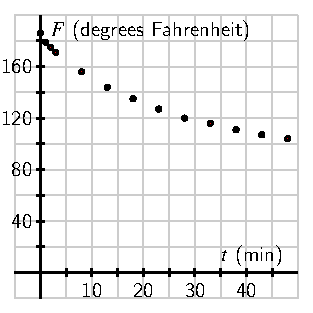
\includegraphics{modeling-exp-coffee}
\end{image}


In one sense, the data looks exponential: the points appear to lie on a curve that is always decreasing and decreasing at an increasing rate.  However, we know that the function can't have the form $f(t) = ab^t$ because such a function's range is the set of all positive real numbers, and it's impossible for the coffee's temperature to fall below room temperature ($71^\circ$).  It is natural to wonder if a function of the form $g(t) = ab^t + c$ will work.  Thus, in order to find a function that fits the data in a situation such as this, we begin by investigating and understanding the roles of $a$, $b$, and $c$ in the behavior of $g(t) = ab^t + c$.

\begin{exploration}
In \link[\emph{Desmos}]{desmos.com}, define $g(t) = ab^t+c$ and accept the prompt for sliders for both $a$ and $b$. Edit the sliders so that $a$ has values from $a = 5$ to $a = 50$, $b$ has values from $b = 0.7$ to $b = 1.3$, and $c$ has values from $c = -5$ to $b = 5$ (also with a step-size of 0.01). In addition, in \emph{Desmos} let $P = (0, g(0))$ and check the box to show the label. Finally, zoom out so that the window shows an interval of $t$-values from $-30 \le t \le 30$
\begin{enumerate}[label=\alph*.]
\item Set $b = 1.1$ and explore the effects of changing the values of $a$ and $c$.  Write several sentences to summarize your observations.
\item Follow the directions for (a) again, this time with $b = 0.9$
\item Set $a = 5$ and $c = 4$. Explore the effects of changing the value of $b$; be sure to include values of $b$ both less than and greater than 1. Write several sentences to summarize your observations.
\item When $0 \lt b \lt 1$, what happens to the graph of $g$ when we consider positive $t$-values that get larger and larger?
\end{enumerate}
\end{exploration}


%\typeout{************************************************}
%\typeout{Long-term behavior of exponential functions}
%\typeout{************************************************}

\section{Long-term behavior of exponential functions}
We have already established that any exponential function of the form $f(t) = ab^t$ where $a$ and $b$ are positive real numbers with $b \ne 1$ is always concave up and is either always increasing or always decreasing.  We next introduce precise language to describe the behavior of an exponential function's value as $t$ gets bigger and bigger.  To start, let's consider the two basic exponential functions $p(t) = 2^t$ and $q(t) = \left(\frac{1}{2}\right)^t$ and their respective values at $t = 10$, $t = 20$, and $t = 30$, as displayed below.
%talks about concave up, which we haven't defined!

$$
%\begin{array}{cccccc}
%$
{\begin{array}{cc}
t&p(t)\\
\hline
10&2^10=1026\\
20&2^20=1048576\\
30&2^30=1073741824
\end{array}}%&&&&& 
$$
%$
%\end{center}
%\begin{center}
%$
$$
{\begin{array}{cc}
t&q(t)\\
\hline
10&\left(\frac{1}{2}\right)^10=\frac{1}{1026} \approx 0.00097656\\
10&\left(\frac{1}{2}\right)^20=\frac{1}{1048576} \approx 0.00000095367\\
10&\left(\frac{1}{2}\right)^30=\frac{1}{1073741824} \approx 0.00000000093192
\end{array}}\\
%\end{array}
$$

For the increasing function $p(t) = 2^t$, we see that the output of the function gets very large very quickly.  In addition, there is no upper bound to how large the function can be.  Indeed, we can make the value of $p(t)$ as large as we'd like by taking $t$ sufficiently big.  We thus say that as $t$ increases, $p(t)$ \dfn{increases without bound}.

For the decreasing function $q(t) =\left(\frac{1}{2}\right)^t$, we see that the output $q(t)$ is always positive but getting closer and closer to $0$.  Indeed, becasue we can make $2^t$ as large as we like, it follows that we can make its reciprocal $\frac{1}{2^t} =\left(\frac{1}{2}\right)^t$ as small as we'd like.  We thus say that as $t$ increases, $q(t)$ \dfn{approaches $0$}. \index{approaching $0$}

To represent these two common phenomena with exponential functions the value increasing without bound or the value approaching $0$, we will use shorthand notation.  First, it is natural to write ``$q(t) \to 0$'' as $t$ increases without bound.  Moreover, since we have the notion of the infinite to represent quantities without bound, we use the symbol for infinity \index{infinity} ($\infty$) and write ``$p(t) \to \infty$'' as $t$ increases without bound in order to indicate that $p(t)$ increases without bound.

In the exploration above, we saw how the value of $b$ affects the steepness of the graph of $f(t) = ab^t$, as well as how all graphs with $b \gt 1$ have the similar increasing behavior, and all graphs with $0 \lt b \lt 1$ have similar decreasing behavior.  For instance, by taking $t$ sufficiently large, we can make $(1.01)^t$ as large as we want; it just takes much larger $t$ to make $(1.01)^t$ big in comparison to $2^t$.  In the same way, we can make $(0.99)^t$ as close to $0$ as we wish by taking $t$ sufficiently big, even though it takes longer for $(0.99)^t$ to get close to $0$ in comparison to $\left(\frac{1}{2}\right)^t$.  For an arbitrary choice of $b$, we can say the following.

\begin{callout}
\textbf{\Large Long-term behavior of exponential functions.}
Let $f(t) = b^t$ with $b \gt 0$ and $b \ne 1$.
\begin{itemize}
\item If $0 \lt b \lt 1$, then $b^t \to 0$ as $t \to \infty$.  We read this notation as ``$b^t$ tends to $0$ as $t$ increases without bound.
\item If $b \gt 1$, then $b^t \to \infty$ as $t \to \infty$.  We read this notation as ``$b^t$ increases without bound as $t$ increases without bound.
\end{itemize}
\end{callout}

In addition, we make a key observation about the use of exponents.  For the function $q(t) = \left(\frac{1}{2}\right)^t$, there are three equivalent ways we may write the function:%
\begin{equation*}
\left( \frac{1}{2} \right)^t = \frac{1}{2^t} = 2^{-t}\text{.}
\end{equation*}
In our work with transformations involving horizontal scaling in \hyperlink{ez-circular-sinusoidal-horiz-reflection}{Exercise~2.4.5.3}, we saw that the graph of $y = h(-t)$ is the reflection of the graph of $y = h(t)$ across the $y$-axis.  Therefore, we can say that the graphs of $p(t) = 2^t$ and $q(t) = \left(\frac{1}{2}\right)^t = 2^{-t}$ are reflections of one another in the $y$-axis since $p(-t) = 2^{-t} = q(t)$.  We see this fact verified in the graph below.

\begin{image}
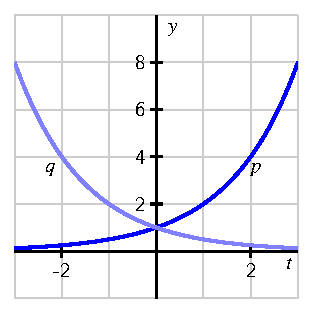
\includegraphics{modeling-exp-reflection}
\end{image}

Similar observations hold for the relationship between the graphs of $b^{t}$ and $\frac{1}{b^t} = b^{-t}$ for any positive $b \ne 1$.


%\typeout{************************************************}
%\typeout{Subsection 3.2.2 The role of $c$ in $g(t) = ab^t + c$}
%\typeout{************************************************}

\section{The role of $c$ in $g(t) = ab^t + c$}

The function $g(t) = ab^t + c$ is a vertical translation of the function $f(t) = ab^t$.  We now have extensive understanding of the behavior of $f(t)$ and how that behavior depends on $a$ and $b$.  Since a vertical translation by $c$ does not change the shape of any graph, we expect that $g$ will exhibit very similar behavior to $f$.  Indeed, we can compare the two functions' graphs as shown in the graphs belowA and then make the following general observations.

\begin{image}
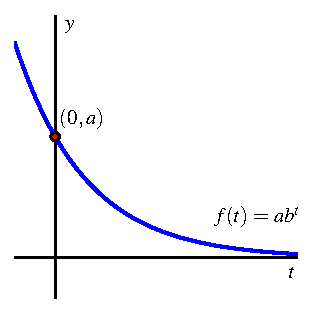
\includegraphics{modeling-vert-transl-0}
\end{image}

\begin{image}
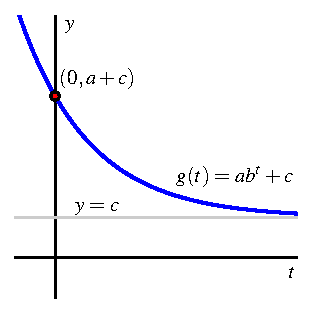
\includegraphics{modeling-vert-transl-c}
\end{image}

\begin{callout}
\textbf{\Large Behavior of vertically shifted exponential functions.}
Let $g(t) = ab^t + c$ with $a \gt 0$, $b \gt 0$ and $b \ne 1$, and $c$ any real number.
\begin{itemize}
\item If $0 \lt b \lt 1$, then $g(t) = ab^t + c \to c$ as $t \to \infty$.  The function $g$ is always decreasing, always concave up, and has $y$-intercept $(0,a+c)$.  The range of the function is all real numbers greater than $c$.
\item If $b \gt 1$, then $g(t) = ab^t + c \to \infty$ as $t \to \infty$.  The function $g$ is always increasing, always concave up, and has $y$-intercept $(0,a+c)$.  The range of the function is all real numbers greater than $c$.
\end{itemize}
\end{callout}


It is also possible to have $a \lt 0$.  In this situation, because $g(t) = ab^t$ is both a reflection of $f(t) = b^t$ across the $x$-axis and a vertical stretch by $|a|$, the function $g$ is always concave down.  If $0 \lt b \lt 1$ so that $f$ is always decreasing, then $g$ is always increasing; if instead $b \gt 1$ so $f$ is increasing, then $g$ is decreasing.  Moreover, instead of the range of the function $g$ having a lower bound as when $a \gt 0$, in this setting the range of $g$ has an upper bound.  These ideas are explored further below.

It's an important skill to be able to look at an exponential function of the form $g(t) = ab^t + c$ and form an accurate mental picture of the graph's main features in light of the values of $a$, $b$, and $c$.

\begin{exploration}
For each of the following functions, \emph{without} using graphing technology, determine whether the function is
\begin{enumerate}[label=\roman*.]
\item always increasing or always decreasing;
\item always concave up or always concave down; and
\item increasing without bound, decreasing without bound, or increasing/decreasing toward a finite value.
\end{enumerate}
In addition, state the $y$-intercept and the range of the function.  For each function, write a sentence that explains your thinking and sketch a rough graph of how the function appears.
\begin{enumerate}[label=\alph*.]
\item $p(t) = 4372 (1.000235)^t + 92856$
\item $q(t) = 27931 (0.97231)^t + 549786$
\item $r(t) = -17398 (0.85234)^t$
\item $s(t) = -17398 (0.85234)^t + 19411$%
\item $u(t) = -7522 (1.03817)^t$%
\item $v(t) = -7522 (1.03817)^t + 6731$%
\end{enumerate}
\end{exploration}


%\typeout{************************************************}
%\typeout{Subsection 3.2.3 Modeling temperature data}
%\typeout{************************************************}

\section{Modeling temperature data}
Newton's Law of Cooling \index{Newton's Law of Cooling} states that the rate that an object warms or cools occurs in direct proportion to the difference between its own temperature and the temperature of its surroundings.  If we return to the coffee temperature data  and recall that the room temperature in that experiment was $71^\circ$, we can see how to use a transformed exponential function to model the data.  In the table below, we add a row of information to the table where we compute $F(t)-71$ to subtract the room temperature from each reading.

$$
\begin{array}{ccc}
\multicolumn{3}{c}{\text{Data for cooling coffee}}\\
\multicolumn{3}{c}{\text{(measured in degrees Fahrenheit at the time t in minutes)}}\\
t&F(t)&f(t)=F(t)-71\\
\hline
0&186&115\\
1&179&108\\
2&175&104\\
3&171&100\\
8&156&85\\
13&144&73\\
18&135&64\\
23&127&56\\
28&120&49\\
33&116&45\\
38&111&40\\
43&107&36\\
48&104&33
\end{array}
$$

The data in the last row of the table appears exponential, and if we test the data by computing the quotients of output values that correspond to equally-spaced input, we see a nearly constant ratio.  In particular,%
\begin{equation*}
\frac{73}{85} \approx 0.86, \ \frac{64}{73} \approx 0.88, \ \frac{56}{64} \approx 0.88, \ \frac{49}{56} \approx 0.88, \ \frac{45}{49} \approx 0.92, \text{and} \frac{40}{45} \approx 0.89 \text{.}
\end{equation*}
Of course there is some measurement error in the data (plus it is only recorded to accuracy of whole degrees), so these computations provide convincing evidence that the underlying function is exponential.  In addition, we expect that if the data continued in the last of the table, the values would approach $0$ because $F(t)$ will approach $71$.

\begin{image}
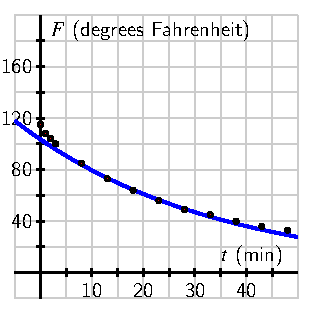
\includegraphics{modeling-coffee-shifted}
\end{image}

\begin{image}
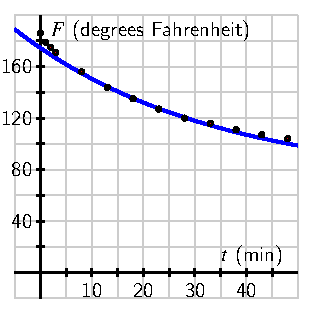
\includegraphics{modeling-coffee-original}
\end{image}

If we choose two of the data points, say $(18,64)$ and $(23,56)$, and assume that $f(t) = ab^t$, we can determine the values of $a$ and $b$.  Doing so, it turns out that $a \approx 103.503$ and $b \approx 0.974$, so $f(t) = 103.503 ( 0.974)^t$.  Since $f(t) = F(t) - 71$, we see that $F(t) = f(t) + 71$, so $F(t) = 103.503 (0.974)^t + 71$.  Plotting $f$ against the shifted data and $F$ along with the original data in the graphs above, we see that the curves go exactly through the points where $t = 18$ and $t = 23$ as expected, but also that the function provides a reasonable model for the observed behavior at any time $t$.  If our data was even more accurate, we would expect that the curve's fit would be even better.

Our preceding work with the coffee data can be done similarly with data for any cooling or warming object whose temperature initially differs from its surroundings.  Indeed, it is possible to show that Newton's Law of Cooling implies that the object's temperature is given by a function of the form $F(t) = ab^t + c$.

\begin{exploration}
A can of soda (at room temperature) is placed in a refrigerator at time $t = 0$ (in minutes) and its temperature, $F(t)$, in degrees Fahrenheit, is computed at regular intervals. Based on the data, a model is formulated for the object's temperature, given by
\begin{equation*}
F(t) = 42 + 30(0.95)^{t}\text{.}
\end{equation*}
\begin{enumerate}[label=\alph*.]
\item Consider the simpler (parent) function $p(t) = (0.95)^t$. How do you expect the graph of this function to appear? How will it behave as time increases? Without using graphing technology, sketch a rough graph of $p$ and write a sentence of explanation.
\item For the slightly more complicated function $r(t) = 30 (0.95)^{t}$, how do you expect this function to look in comparison to $p$?  What is the long-range behavior of this function as $t$ increases? Without using graphing technology, sketch a rough graph of $r$ and write a sentence of explanation.
\item Finally, how do you expect the graph of $F(t) = 42 + 30(0.95)^{t}$ to appear? Why?  First sketch a rough graph without graphing technology, and then use technology to check your thinking and report an accurate, labeled graph on the axes provided.
\begin{image}
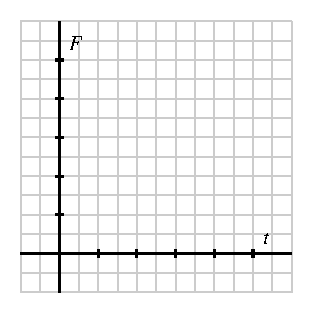
\includegraphics{modeling-F-t-blank-axes}
\end{image}
\item What is the temperature of the refrigerator? What is the room temperature of the surroundings outside the refrigerator? Why?
\item Determine the average rate of change of $F$ on the intervals $[10,20]$, $[20,30]$, and $[30,40]$. Write at least two careful sentences that explain the meaning of the values you found, including units, and discuss any overall trend in how the average rate of change is changing.
\end{enumerate}
\end{exploration}


\begin{exploration}
A potato initially at room temperature ($68^\circ$) is placed in an oven (at $350^\circ$) at time $t = 0$. It is known that the potato's temperature at time $t$ is given by the function $F(t) = a - b(0.98)^t$ for some positive constants $a$ and $b$, where $F$ is measured in degrees Fahrenheit and $t$ is time in minutes.

\begin{enumerate}[label=\alph*.]
\item What is the numerical value of $F(0)$? What does this tell you about the value of $a - b$?
\item Based on the context of the problem, what should be the long-range behavior of the function $F(t)$? Use this fact along with the behavior of $(0.98)^t$ to determine the value of $a$.  Write a sentence to explain your thinking.
\item What is the value of $b$?  Why?%
\item Check your work above by plotting the function $F$ using graphing technology in an appropriate window. Record your results on the axes provided, labeling the scale on the axes. Then, use the graph to estimate the time at which the potato's temperature reaches $325$ degrees.
\begin{image}
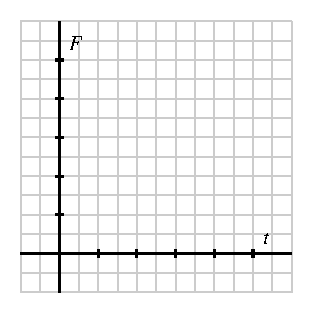
\includegraphics{modeling-F-t-blank-axes}
\end{image}
\item How can we view the function $F(t) = a - b(0.98)^t$ as a transformation of the parent function $f(t) = (0.98)^t$?  Explain.
\end{enumerate}
\end{exploration}

\begin{summary}\begin{itemize}
\item For an exponential function of the form $f(t) = b^t$, the function either approaches zero or grows without bound as the input gets larger and larger.  In particular, if $0 \lt b \lt 1$, then $f(t) = b^t \to 0$ as $t \to \infty$, while if $b \gt 1$, then $f(t) = b^t \to \infty$ as $t \to \infty$.  Scaling $f$ by a positive value $a$ (that is, the transformed function $ab^t$) does not affect the long-range behavior:  whether the function tends to $0$ or increases without bound depends solely on whether $b$ is less than or greater than $1$.%
\item{}\hypertarget{p-1350}{}%
The function $f(t) = b^t$ passes through $(0,1)$, is always concave up, is either always increasing or always decreasing, and its range is the set of all positive real numbers.  Among these properties, a vertical stretch by a positive value $a$ only affects the $y$-intercept, which is instead $(0,a)$.  If we include a vertical shift and write $g(t) = ab^t + c$, the biggest changes is that the range of $g$ is the set of all real numbers greater than $c$.  In addition, the $y$-intercept of $g$ is $(0,a+c)$.
\item In the situation where $a \lt 0$, several other changes are induced.  Here, because $g(t) = ab^t$ is both a reflection of $f(t) = b^t$ across the $x$-axis and a vertical stretch by $|a|$, the function $g$ is now always concave down.  If $0 \lt b \lt 1$ so that $f$ is always decreasing, then $g$ (the reflected function) is now always increasing; if instead $b \gt 1$ so $f$ is increasing, then $g$ is decreasing.  Finally, if $a \lt 0$, then the range of $g(t) = ab^t + c$ is the set of all real numbers $c$.
\item An exponential function can be thought of as a function that changes at a rate proportional to itself, like how money grows with compound interest or the amount of a radioactive quantity decays.  Newton's Law of Cooling says that the rate of change of an object's temperature is proportional to the \emph{difference} between its own temperature and the temperature of its surroundings.  This leads to the function that measures the difference between the object's temperature and room temperature being exponential, and hence the object's temperature itself is a vertically-shifted exponential function of the form $F(t) = ab^t + c$.
\end{itemize}\end{summary}

\end{document}
